\chapter{Arquitectura} % Chapter title

\label{ch:arquitectura} % For referencing the chapter elsewhere, use \autoref{ch:introduccion} 

%----------------------------------------------------------------------------------------
\graffito{A cada uno de los servicios enunciados en este informe le corresponde una carpeta dentro del repositorio del proyecto. El código fuente es de acceso libre y se encuentra en \url{https://github.com/sebastianaf/pricecloud}.\bigskip}

\section{Esquema de servicios}

\begin{center}
    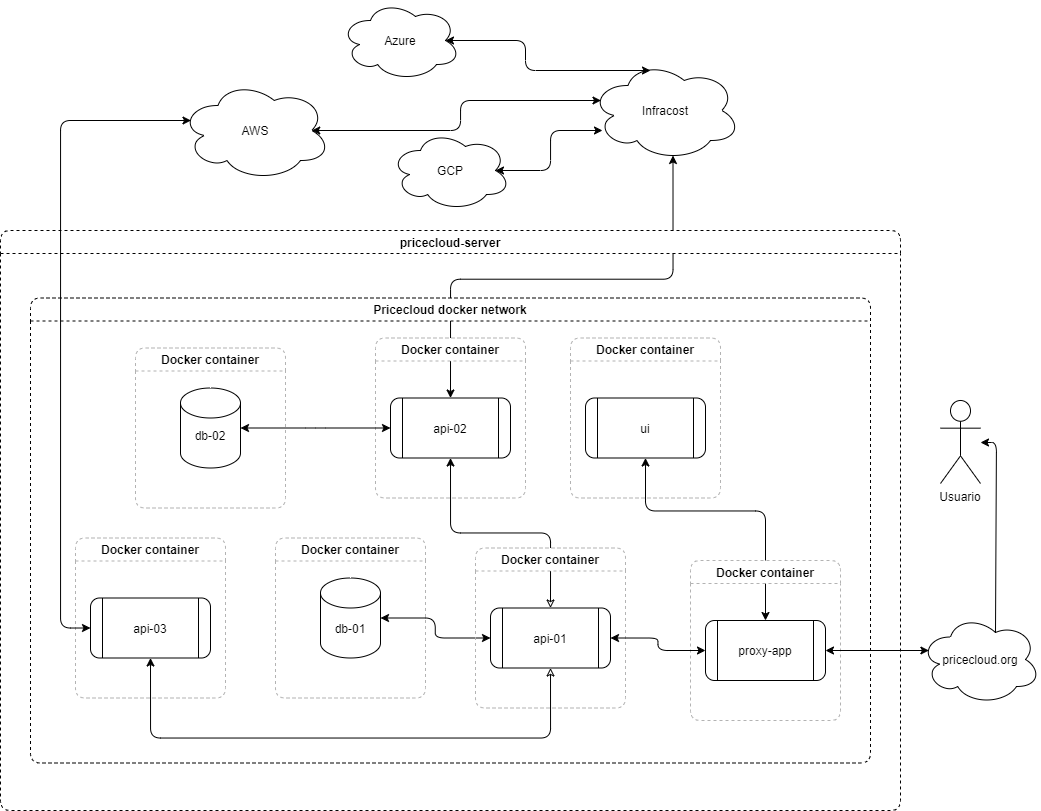
\includegraphics[width=\textwidth]{gfx/services.drawio.png}
\end{center}

\section{Descripción de los servicios}
La aplicación esta compuesta por seis microservicios con funciones específicas cada uno descritas a continuación.

\subsection{\acrshort{API REST} \emph{api-01}} (NestJS)
El primer microservicio del backend se encarga de autenticar los usuarios de la aplicación y centralizar todas las peticiones. Este servicio está expuesto en Internet en \url{https://api.pricecloud.org} y su documentación está en \url{https://api.dev.pricecloud.org} se comunica usando el protocolo \acrshort{HTTPS} gracias a que se encuentra detrás del contenedor de \gls{Nginx Proxy Manager},también esta comunicado con \emph{api-03} para el aprovisionamiento de servicios
en \acrshort{AWS}, con \emph{ui} autenticando cada petición con \emph{JSON Web Tokens} cifrados con \acrfull{AES}; La responsabilidad de este servicio es responder todas las peticiones creadas por el frontend de la aplicación incluyendo las consultas de los precios de los \acrfullpl{CCSP} almacenadas en la base de datos \emph{db-02} accedida por \emph{api-02}.

\subsection{\acrshort{API REST} \emph{api-02}} (ApolloServer)
El segundo microservicio de backend se encarga de recopilar la información de precios de los \acrshortpl{CCSP}. Este sevicio accede a la data de \emph{db-02} donde hay mas de 3 millones de registros de precios de \acrshortpl{CCSP}, esta parte de la aplicación también tiene la responsabilidad de actualizar la base de datos de precio cuando \emph{api-01} se lo indique, esta actualización es una consulta a los servidores de \emph{Infracost} accediendo a la base de datos libre de precios.

\subsection{\acrshort{API REST} \emph{api-03}} (Python Flask)
El tercer microservicio de backend se encarga de aprovisionar recursos en \acrshort{AWS} usando \gls{LibCloud} para la creación de instancias \emph{EC2} y \emph{S3}.

\subsection{Base de datos \emph{db-01}} (PostgreSQL)
Este microservicio corresponde a la base de datos principal del proyecto, aquí residen los datos de todos los usuarios, sus roles y permisos el esquema de datos de este servidor esta definido en \emph{api-01} por \gls{TypeORM}.

\subsection{Base de datos \emph{db-02}} (PostgreSQL)
Por motivos de rendimiento se decidió separar la base de datos de precios de los \acrshortpl{CCSP} en un servidor aparte, esta base de datos es accedida por \emph{api-02} y se actualiza semanalmente por \emph{api-02}.

\subsection{Interfaz Web \emph{ui}} (NextJS)
Este servicio se encarga de ejecutar el servidor web con la interfaz gráfica de usuario. Implementa un esquema de autenticación por \emph{cookies} con tokens \emph{JWT} encriptados con \acrshortpl{AES}, este microservicio se comunica con \emph{api-01} para solicitar todas las funcionalidades de la aplicaciones al resto de los contenedores. Esta parte de la aplicación es accesible en

%----------------------------------------------------------------------------------------
